\documentclass[8pt]{beamer}

\usepackage{threeparttable}
\usepackage{array}
\usepackage{graphicx}
\usepackage{tabularx}
\usepackage{booktabs}




\begin{document}

\begin{frame}{Summary statistics}
	I have regenerated the summary statistics.  There is a small change, and it should be reflected in the paper. This table is not formatted as well as the one in the paper, but the layout is exactly the same, so it should be quick to cut and paste into the paper.
	
	\begin{table}[!htbp] \centering \renewcommand*{\arraystretch}{1.1}\caption{Summary statistics\label{tab:sumstat}}\resizebox{\textwidth}{!}{
\begin{tabular}{lrrrrrr}
\hline
\hline
non\_participant & \multicolumn{3}{c}{No} & \multicolumn{3}{c}{Yes}  \\ 
 Variable & \multicolumn{1}{c}{N} & \multicolumn{1}{c}{Mean} & \multicolumn{1}{c}{SD} & \multicolumn{1}{c}{N} & \multicolumn{1}{c}{Mean} & \multicolumn{1}{c}{SD} \\ 
\hline
Energy consumption data & 0 &  &  & 0 &  &  \\ 
Actual gas consumption (GJ/year) & 1453 & 113 & 38 & 18284 & 116 & 41 \\ 
Actual electricity consumption (GJ/year) & 1453 & 31 & 12 & 18284 & 31 & 13 \\ 
Actual energy consumption (GJ/year) & 1453 & 144 & 45 & 18284 & 148 & 48 \\ 
Property assessment data & 0 &  &  & 0 &  &  \\ 
Total assessed value (\$) & 1453 & 276665 & 87090 & 18284 & 289405 & 123025 \\ 
Lot size (square metres) & 1453 & 642 & 294 & 18284 & 816 & 1875 \\ 
Building size (square metres) & 1453 & 118 & 39 & 18284 & 121 & 43 \\ 
Year built & 1453 & 1971 & 18 & 18284 & 1981 & 23 \\ 
Program participation data & 0 &  &  & 0 &  &  \\ 
Air sealing & 1453 & 0.82 & 0.38 & 18284 & 0 & 0 \\ 
Attic insulation & 1453 & 0.64 & 0.48 & 18284 & 0 & 0 \\ 
Wall insulation & 1453 & 0.044 & 0.21 & 18284 & 0 & 0 \\ 
Basement insulation & 1453 & 0.13 & 0.33 & 18284 & 0 & 0 \\ 
Foundation header insulation & 1453 & 0.087 & 0.28 & 18284 & 0 & 0 \\ 
Window or door upgrade & 1453 & 0.18 & 0.39 & 18284 & 0 & 0 \\ 
Central A/C upgrade & 1453 & 0.13 & 0.34 & 18284 & 0 & 0 \\ 
Natural gas furnace upgrade & 1453 & 0.68 & 0.47 & 18284 & 0 & 0 \\ 
Predicted pre-retrofit gas consumption (GJ/year) & 1453 & 161 & 60 & 0 &  &  \\ 
Predicted pre-retrofit electricity consumption (GJ/year) & 1453 & 34 & 1 & 0 &  &  \\ 
Predicted pre-retrofit energy consumption (GJ/year) & 1453 & 195 & 60 & 0 &  &  \\ 
Predicted post-retrofit gas consumption (GJ/year) & 1453 & 116 & 40 & 0 &  &  \\ 
Predicted post-retrofit electricity consumption (GJ/year) & 1453 & 33 & 1.1 & 0 &  &  \\ 
Predicted post-retrofit energy consumption (GJ/year) & 1453 & 149 & 40 & 0 &  & \\ 
\hline
\hline
\end{tabular}
}
\end{table}


\end{frame}

\begin{frame}{Introduction}
	The first results section should discuss research design, with a focus on sample selection. De we want the \textit{full sample}? A \textit{matched sample} consisting of the treated group and matched controls? The \textit{treated group only}? Each of these different approaches has been used in prior research (cite).  Each has different things to recommend and detract. With untreated controls, we can estimate the treatment effect over a longer window. We also can be less worried about ``forbidden regressions'' that compare later treated with earlier treated units. However, with untreated units as controls, we may be more concerned about selection.  The first section should elaborate on this discussion, with citations, and produce results.    I present results in the following tables.
	
	Unless otherwise stated, column definitions are as follows
	\begin{enumerate}
		\item Treated + all available controls
		\item Treated + 1:1 matched controls based on pre-treatment consumption
		\item Treated + 1:1 matched controls based on building characteristics
		\item Treated + 1:1 matched controls based on pre-treatment consumption and building characteristics
		\item Treated only
	\end{enumerate}

	Note that in the `Treated only'' samples, I only follow units until 2011. After 2012, all units are treated.
	
	Note that we do not need all of the tables that follow. I put them here for completeness (some may be dropped or go in appendix).
\end{frame}

\begin{frame}{TWFE estimates for total energy; monthly data}
	
\begingroup
\centering
\begin{tabular}{lccccc}
   \tabularnewline \midrule \midrule
   Dependent Variable: & \multicolumn{5}{c}{log(energy)}\\
   Model:             & (1)             & (2)             & (3)             & (4)             & (5)\\  
   \midrule
   \emph{Variables}\\
   treated\_postTRUE  & -0.1571$^{***}$ & -0.1453$^{***}$ & -0.1512$^{***}$ & -0.1396$^{***}$ & -0.1573$^{***}$\\   
                      & (0.0063)        & (0.0072)        & (0.0070)        & (0.0074)        & (0.0107)\\   
   \midrule
   \emph{Fixed-effects}\\
   id                 & Yes             & Yes             & Yes             & Yes             & Yes\\  
   cons\_date         & Yes             & Yes             & Yes             & Yes             & Yes\\  
   \midrule
   \emph{Fit statistics}\\
   Observations       & 2,882,662       & 429,578         & 429,833         & 429,866         & 75,461\\  
   R$^2$              & 0.79219         & 0.80557         & 0.81004         & 0.81181         & 0.81352\\  
   Within R$^2$       & 0.00267         & 0.01011         & 0.01134         & 0.00962         & 0.01377\\  
   \midrule \midrule
   \multicolumn{6}{l}{\emph{Clustered (id \& cons\_date) standard-errors in parentheses}}\\
   \multicolumn{6}{l}{\emph{Signif. Codes: ***: 0.01, **: 0.05, *: 0.1}}\\
\end{tabular}
\par\endgroup



\end{frame}

\begin{frame}{TWFE estimates for gas; monthly data}
	
\begingroup
\centering
\begin{tabular}{lccccc}
   \tabularnewline \midrule \midrule
   Dependent Variable: & \multicolumn{5}{c}{log(gas)}\\
   Model:             & (1)             & (2)             & (3)             & (4)             & (5)\\  
   \midrule
   \emph{Variables}\\
   treated\_postTRUE  & -0.2081$^{***}$ & -0.1944$^{***}$ & -0.1993$^{***}$ & -0.1901$^{***}$ & -0.2196$^{***}$\\   
                      & (0.0062)        & (0.0076)        & (0.0074)        & (0.0078)        & (0.0089)\\   
   \midrule
   \emph{Fixed-effects}\\
   id                 & Yes             & Yes             & Yes             & Yes             & Yes\\  
   cons\_date         & Yes             & Yes             & Yes             & Yes             & Yes\\  
   \midrule
   \emph{Fit statistics}\\
   Observations       & 2,874,433       & 428,688         & 429,313         & 429,103         & 75,699\\  
   R$^2$              & 0.85408         & 0.85549         & 0.85894         & 0.86033         & 0.84099\\  
   Within R$^2$       & 0.00384         & 0.01381         & 0.01480         & 0.01352         & 0.01773\\  
   \midrule \midrule
   \multicolumn{6}{l}{\emph{Clustered (id \& cons\_date) standard-errors in parentheses}}\\
   \multicolumn{6}{l}{\emph{Signif. Codes: ***: 0.01, **: 0.05, *: 0.1}}\\
\end{tabular}
\par\endgroup



\end{frame}

\begin{frame}{TWFE estimates for electricity; monthly data}
	
\begingroup
\centering
\begin{tabular}{lccccc}
   \tabularnewline \midrule \midrule
   Dependent Variable: & \multicolumn{5}{c}{log(elec)}\\
   Model:             & (1)                   & (2)                   & (3)                   & (4)                   & (5)\\  
   \midrule
   \emph{Variables}\\
   treated\_postTRUE  & -0.0387$^{***}$       & -0.0138               & -0.0084               & 0.0015                & 0.0207\\   
                      & (0.0099)              & (0.0121)              & (0.0123)              & (0.0117)              & (0.0155)\\   
   \midrule
   \emph{Fixed-effects}\\
   id                 & Yes                   & Yes                   & Yes                   & Yes                   & Yes\\  
   cons\_date         & Yes                   & Yes                   & Yes                   & Yes                   & Yes\\  
   \midrule
   \emph{Fit statistics}\\
   Observations       & 2,908,550             & 432,238               & 432,263               & 432,424               & 76,430\\  
   R$^2$              & 0.46709               & 0.50410               & 0.49463               & 0.49444               & 0.54453\\  
   Within R$^2$       & $8.72\times 10^{-5}$  & $5.66\times 10^{-5}$  & $2.07\times 10^{-5}$  & $7.29\times 10^{-7}$  & 0.00014\\  
   \midrule \midrule
   \multicolumn{6}{l}{\emph{Clustered (id \& cons\_date) standard-errors in parentheses}}\\
   \multicolumn{6}{l}{\emph{Signif. Codes: ***: 0.01, **: 0.05, *: 0.1}}\\
\end{tabular}
\par\endgroup



\end{frame}

\begin{frame}{Sun + Abraham estimates}
	The Sun and Abraham correction (like the Callaway and Sant'Anna corection) is estimated by interacting a cohort dummy with a time-to-treatment dummy. In our monthly data, we observe 49 different ``cohorts'' (i.e., households retrofit in 49 different months).  Our data has 200 different ``time to treatments'' (i.e., months before and after retrofit). This implies estimating a model with about 10,000 dummy variables.  This is not feasible. Instead, to estimate the Sun and Abraham model, I convert to annual data first. The results first show the TWFE estimates based on annual data, to confirm that this does not meaningfully disturb the results.
\end{frame}

\begin{frame}{TWFE estimates for energy; annual data}
	
\begingroup
\centering
\begin{tabular}{lccccc}
   \tabularnewline \midrule \midrule
   Dependent Variable: & \multicolumn{5}{c}{log(energy)}\\
   Model:             & (1)             & (2)             & (3)             & (4)             & (5)\\  
   \midrule
   \emph{Variables}\\
   treated\_postTRUE  & -0.1682$^{***}$ & -0.1573$^{***}$ & -0.1605$^{***}$ & -0.1489$^{***}$ & -0.1870$^{***}$\\   
                      & (0.0060)        & (0.0079)        & (0.0077)        & (0.0090)        & (0.0114)\\   
   \midrule
   \emph{Fixed-effects}\\
   id                 & Yes             & Yes             & Yes             & Yes             & Yes\\  
   consyear           & Yes             & Yes             & Yes             & Yes             & Yes\\  
   \midrule
   \emph{Fit statistics}\\
   Observations       & 246,541         & 35,175          & 35,165          & 35,178          & 5,071\\  
   R$^2$              & 0.80826         & 0.84582         & 0.85472         & 0.85053         & 0.90145\\  
   Within R$^2$       & 0.01388         & 0.06664         & 0.07291         & 0.06048         & 0.11563\\  
   \midrule \midrule
   \multicolumn{6}{l}{\emph{Clustered (id \& consyear) standard-errors in parentheses}}\\
   \multicolumn{6}{l}{\emph{Signif. Codes: ***: 0.01, **: 0.05, *: 0.1}}\\
\end{tabular}
\par\endgroup



\end{frame}

\begin{frame}{Sun+Abraham estimates for energy; annual data}
	
\begingroup
\centering
\begin{tabular}{lccccc}
   \tabularnewline \midrule \midrule
   Dependent Variable: & \multicolumn{5}{c}{log(energy)}\\
   Model:       & (1)             & (2)             & (3)             & (4)             & (5)\\  
   \midrule
   \emph{Variables}\\
   ATT          & -0.1668$^{***}$ & -0.1544$^{***}$ & -0.1577$^{***}$ & -0.1468$^{***}$ & -0.1725$^{***}$\\   
                & (0.0037)        & (0.0049)        & (0.0047)        & (0.0048)        & (0.0155)\\   
   \midrule
   \emph{Fixed-effects}\\
   id           & Yes             & Yes             & Yes             & Yes             & Yes\\  
   consyear     & Yes             & Yes             & Yes             & Yes             & Yes\\  
   \midrule
   \emph{Fit statistics}\\
   Observations & 246,541         & 35,175          & 35,165          & 35,178          & 5,071\\  
   R$^2$        & 0.80831         & 0.84640         & 0.85521         & 0.85139         & 0.90159\\  
   Within R$^2$ & 0.01414         & 0.07016         & 0.07603         & 0.06588         & 0.11683\\  
   \midrule \midrule
   \multicolumn{6}{l}{\emph{Clustered (id \& consyear) standard-errors in parentheses}}\\
   \multicolumn{6}{l}{\emph{Signif. Codes: ***: 0.01, **: 0.05, *: 0.1}}\\
\end{tabular}
\par\endgroup



\end{frame}

\begin{frame}{Sun+Abraham estimates for gas; annual data}
	
\begingroup
\centering
\begin{tabular}{lccccc}
   \tabularnewline \midrule \midrule
   Dependent Variable: & \multicolumn{5}{c}{log(gas)}\\
   Model:       & (1)             & (2)             & (3)             & (4)             & (5)\\  
   \midrule
   \emph{Variables}\\
   ATT          & -0.1958$^{***}$ & -0.1848$^{***}$ & -0.1890$^{***}$ & -0.1781$^{***}$ & -0.2028$^{***}$\\   
                & (0.0042)        & (0.0055)        & (0.0053)        & (0.0054)        & (0.0165)\\   
   \midrule
   \emph{Fixed-effects}\\
   id           & Yes             & Yes             & Yes             & Yes             & Yes\\  
   consyear     & Yes             & Yes             & Yes             & Yes             & Yes\\  
   \midrule
   \emph{Fit statistics}\\
   Observations & 247,154         & 35,234          & 35,244          & 35,248          & 5,071\\  
   R$^2$        & 0.82162         & 0.84958         & 0.86034         & 0.85334         & 0.89767\\  
   Within R$^2$ & 0.01857         & 0.08732         & 0.09513         & 0.08423         & 0.14043\\  
   \midrule \midrule
   \multicolumn{6}{l}{\emph{Clustered (id \& consyear) standard-errors in parentheses}}\\
   \multicolumn{6}{l}{\emph{Signif. Codes: ***: 0.01, **: 0.05, *: 0.1}}\\
\end{tabular}
\par\endgroup



\end{frame}

\begin{frame}{Sun+Abraham estimates for electricity; annual data}
	
\begingroup
\centering
\begin{tabular}{lccccc}
   \tabularnewline \midrule \midrule
   Dependent Variable: & \multicolumn{5}{c}{log(elec)}\\
   Model:       & (1)             & (2)            & (3)           & (4)      & (5)\\  
   \midrule
   \emph{Variables}\\
   ATT          & -0.0495$^{***}$ & -0.0265$^{**}$ & -0.0195$^{*}$ & -0.0146  & 0.0068\\   
                & (0.0071)        & (0.0093)       & (0.0101)      & (0.0093) & (0.0310)\\   
   \midrule
   \emph{Fixed-effects}\\
   id           & Yes             & Yes            & Yes           & Yes      & Yes\\  
   consyear     & Yes             & Yes            & Yes           & Yes      & Yes\\  
   \midrule
   \emph{Fit statistics}\\
   Observations & 246,819         & 35,183         & 35,170        & 35,180   & 5,071\\  
   R$^2$        & 0.64327         & 0.70877        & 0.70024       & 0.70385  & 0.86097\\  
   Within R$^2$ & 0.00060         & 0.00172        & 0.00150       & 0.00112  & 0.00091\\  
   \midrule \midrule
   \multicolumn{6}{l}{\emph{Clustered (id \& consyear) standard-errors in parentheses}}\\
   \multicolumn{6}{l}{\emph{Signif. Codes: ***: 0.01, **: 0.05, *: 0.1}}\\
\end{tabular}
\par\endgroup



\end{frame}

\begin{frame}{Event study plot}
	The next results section should be the event study plot. Here, we emphasize the new estimators, and the potential problems with TWFE.  We can show that the TWFE estimator with participants only results in a very problematic estimate. We should explain that this is because it puts a lot of weight on comparisons between later-treated households and earlier-treated households -- this is a problematic comparison.  All other estimators deliver very similar estimates.
	
	The event study plot suggests that the effect of treatment is highly persistent. Even after 10 years, it looks like savings of about 15 percent are sustained.
\end{frame}

\begin{frame}{Event study plot}
	\centering
	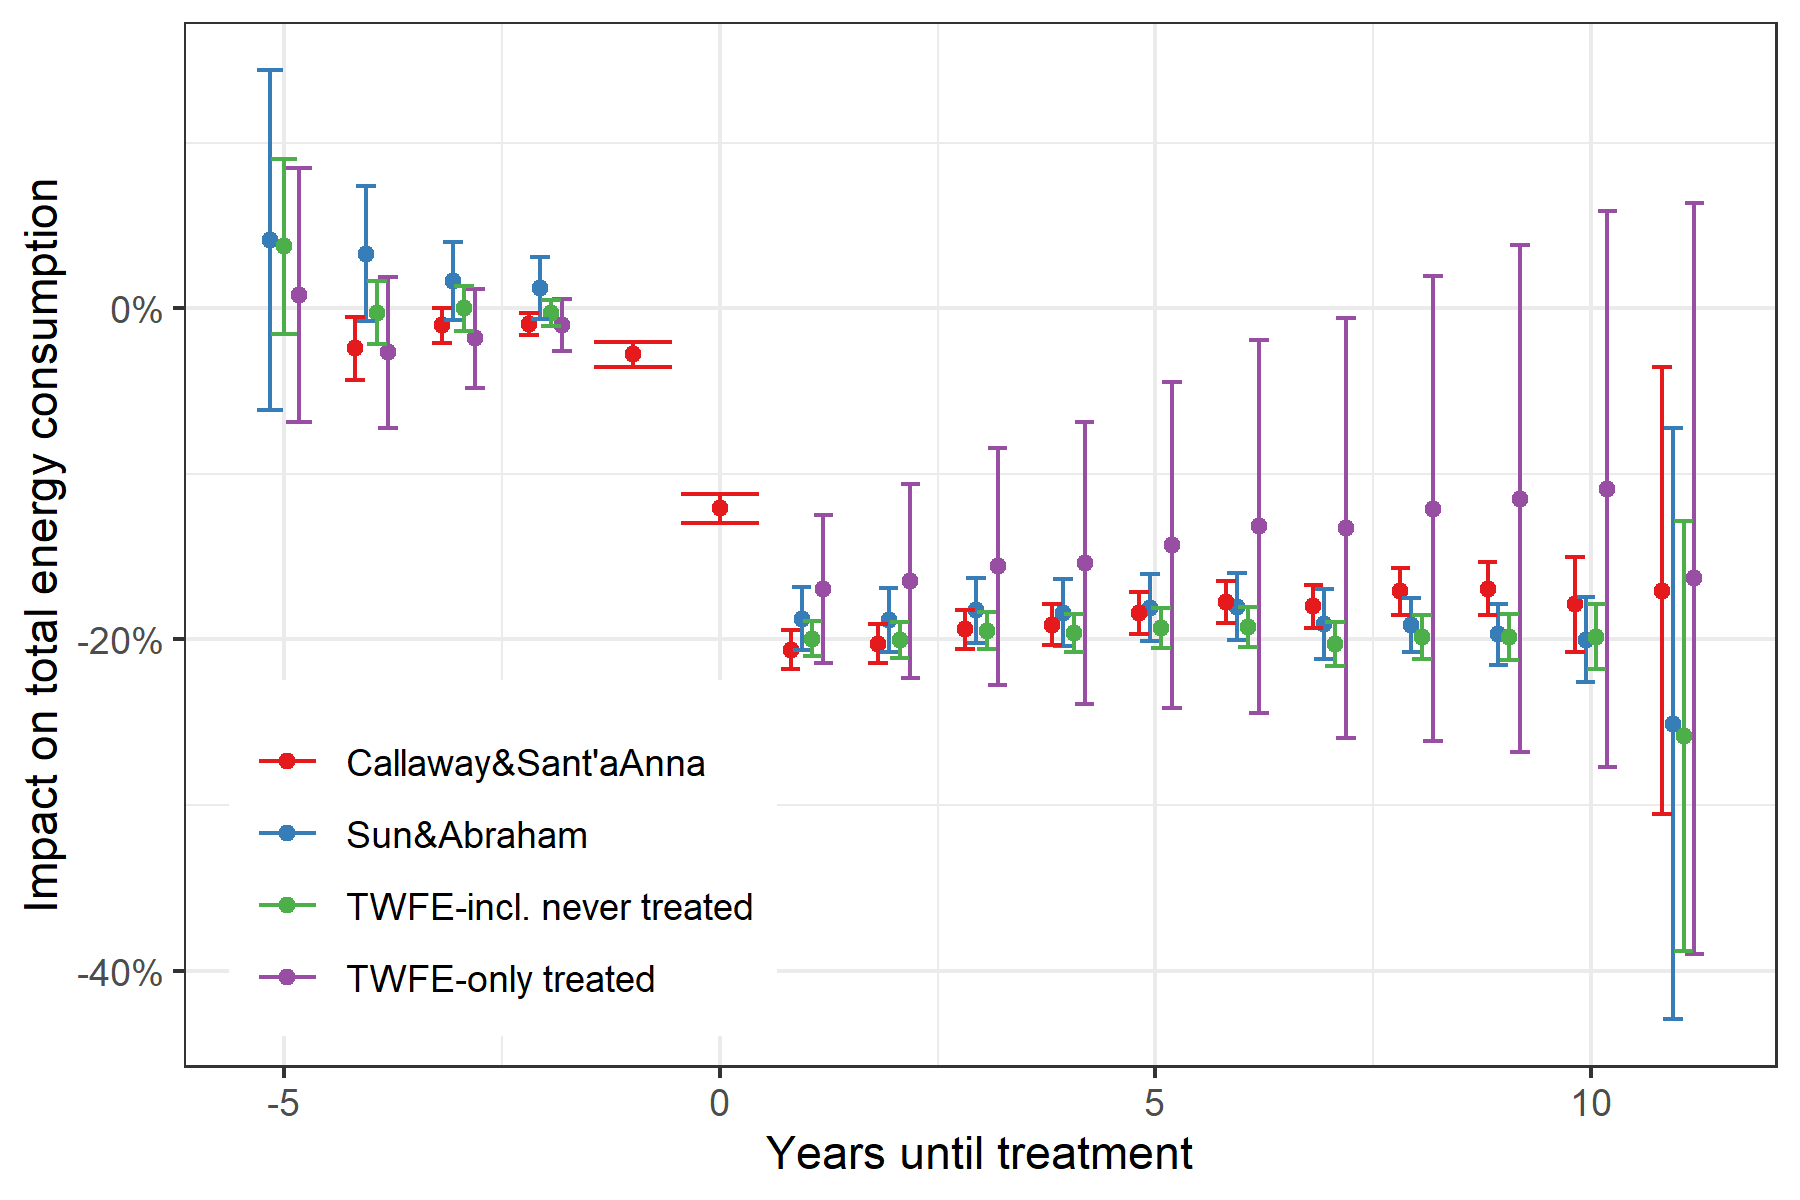
\includegraphics[width=0.75\linewidth]{../output_figures_tables/event_study_plot.png}
\end{frame}


\begin{frame}{Measure by measure results}
	As before, we produce measure-by-measure estimates of savings.
\end{frame}

\begin{frame}{Measure by measure results}
	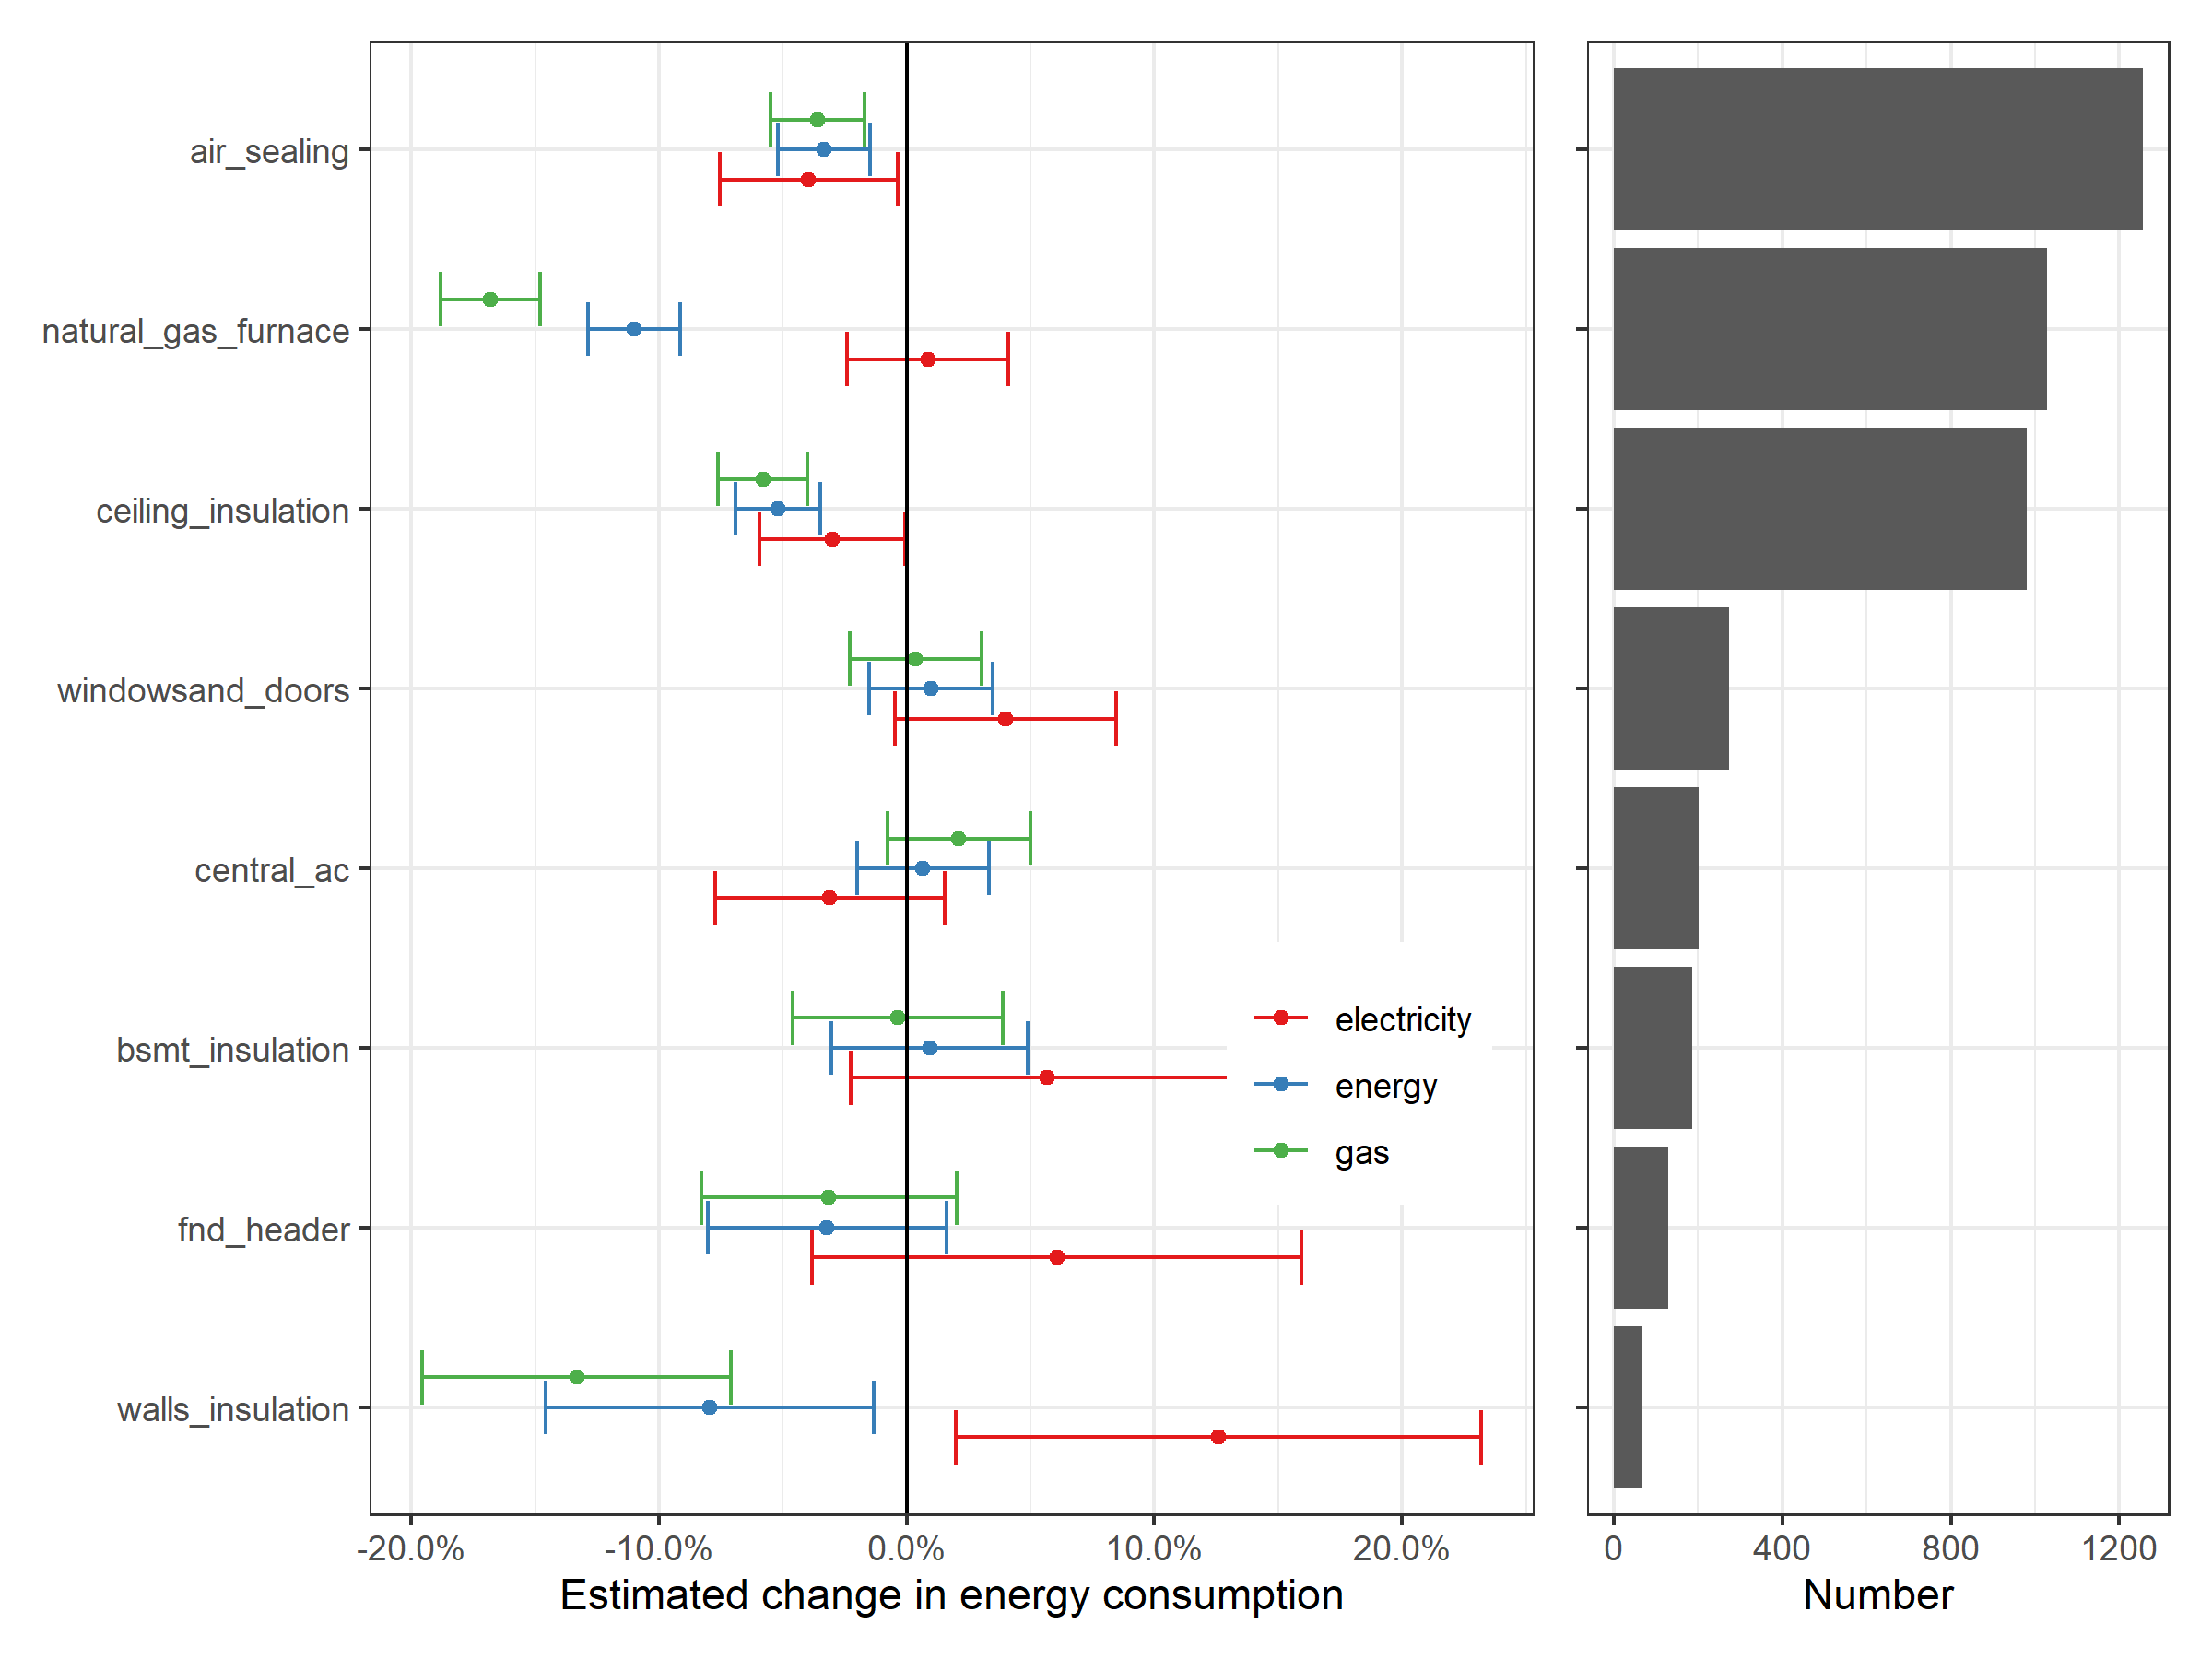
\includegraphics[width=\linewidth]{../output_figures_tables/mbm_energy_savings_combined}
\end{frame}

\begin{frame}{Complete envelope retrofits}
	In the prior figure, we estimate complete energy retrofits using a linear combination of individual measures. Specific measures are listed in the current version of the paper.
	
	I have now added code to use the houses that acutally undergo a complete energy retrofit in order to estimate savings from this combination of measures.  Specifically, I define a complete energy retrofit as:
	\begin{align*}
		\text{complete envelope retrofit} = \\
		\text{air sealing} +
		\text{attic insulation} + \\
		\text{window/door upgrade} +
		\text{wall insulation} + \\
		(\text{foundation header insulation} \text{ OR } \text{basement insulation})
	\end{align*}

	(Note that this is very slightly different from our imputed measure, which adds foundation header AND basement insulation to the other coefficients.)

	There are a total of 15 homes that undergo this definition of a complete energy retrofit. To estimate the effect of this measure, I run a regression on a sample of these homes and untreated homes (and drop all homes that undergo some other retrofit). I control for gas furnace upgrades in this regression.
\end{frame}

\begin{frame}{Complate envelope retrofits}
	Very similar estimates (except for electricity). Could either mention this, or insert the figure directly in the appendix.
	
	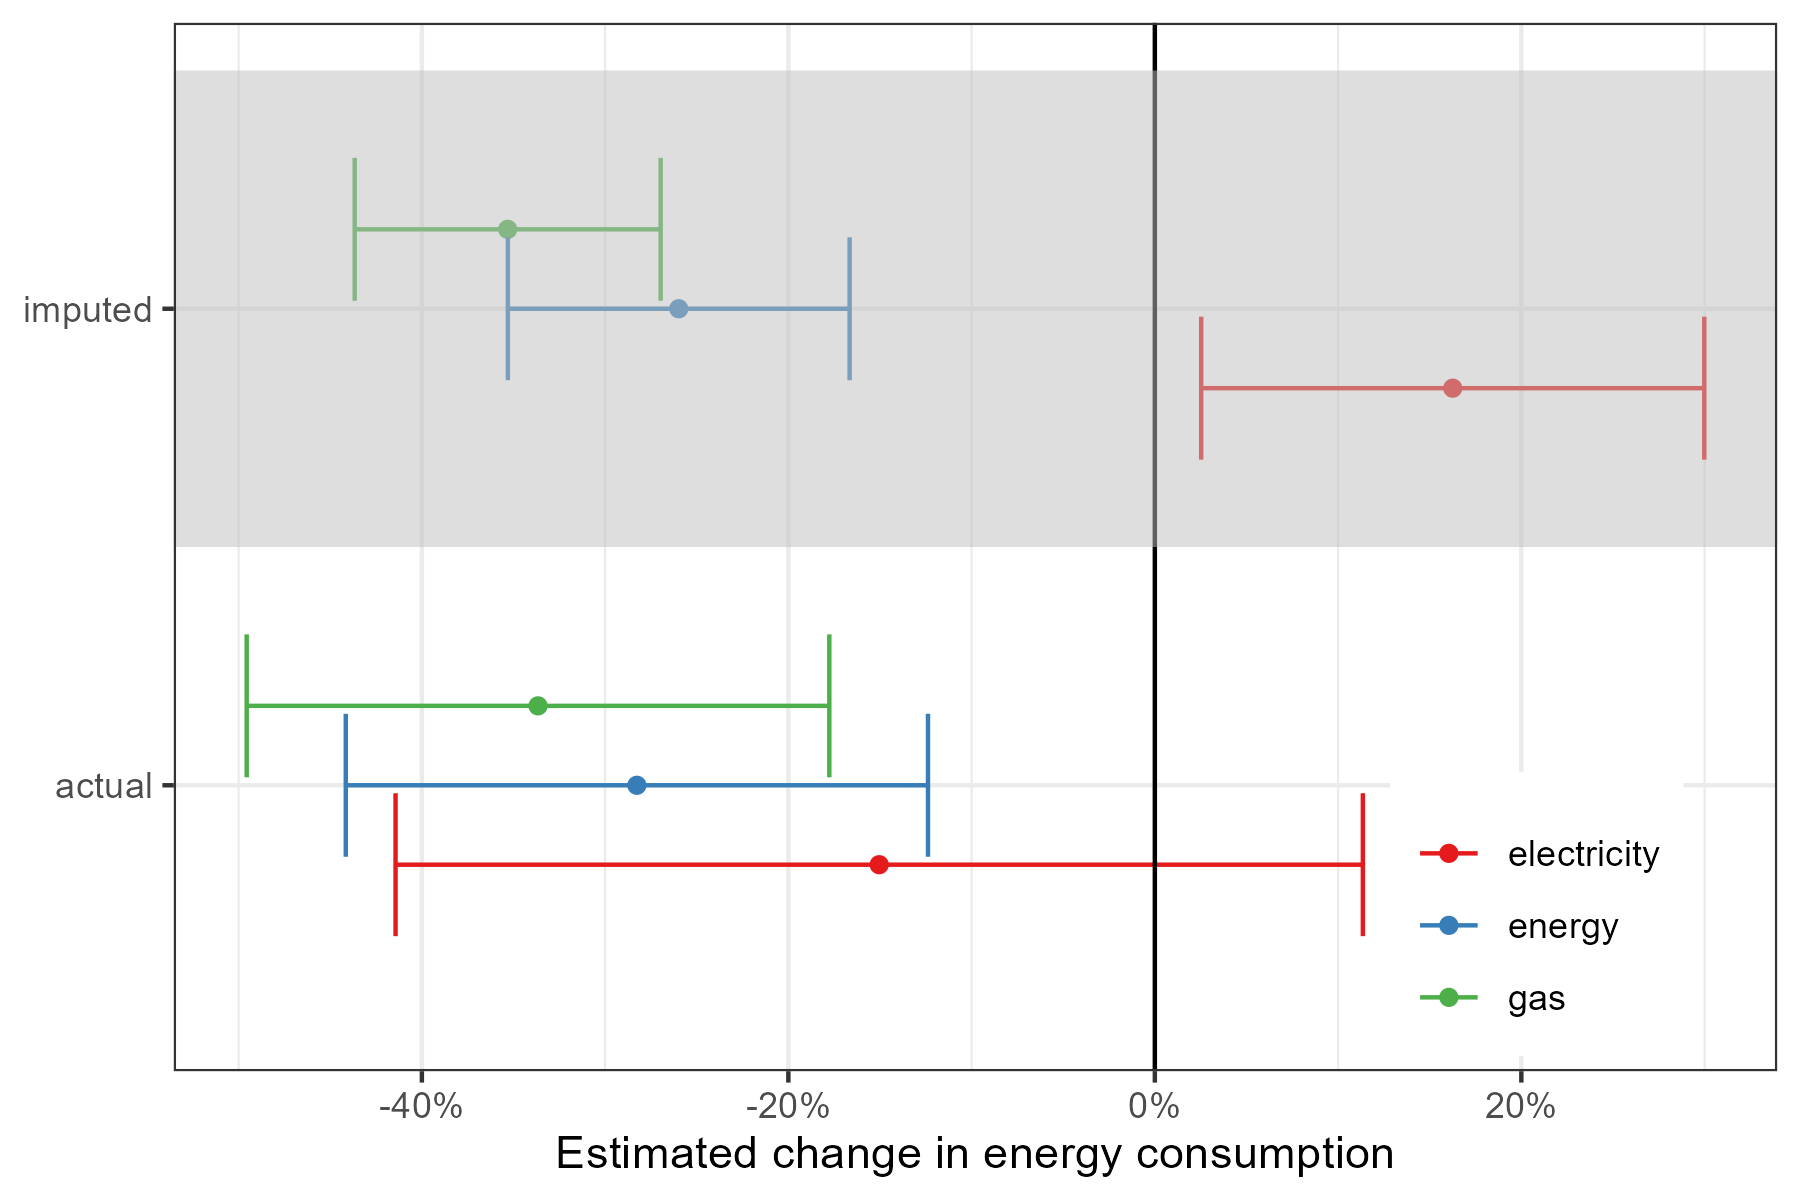
\includegraphics[width=\linewidth]{../output_figures_tables/cer_energy_savings}
\end{frame}

\begin{frame}{Projected energy savings}
	We estimate \textit{projected} energy savings using a cross-sectional regression of projected energy savings on recommended measures.
	
		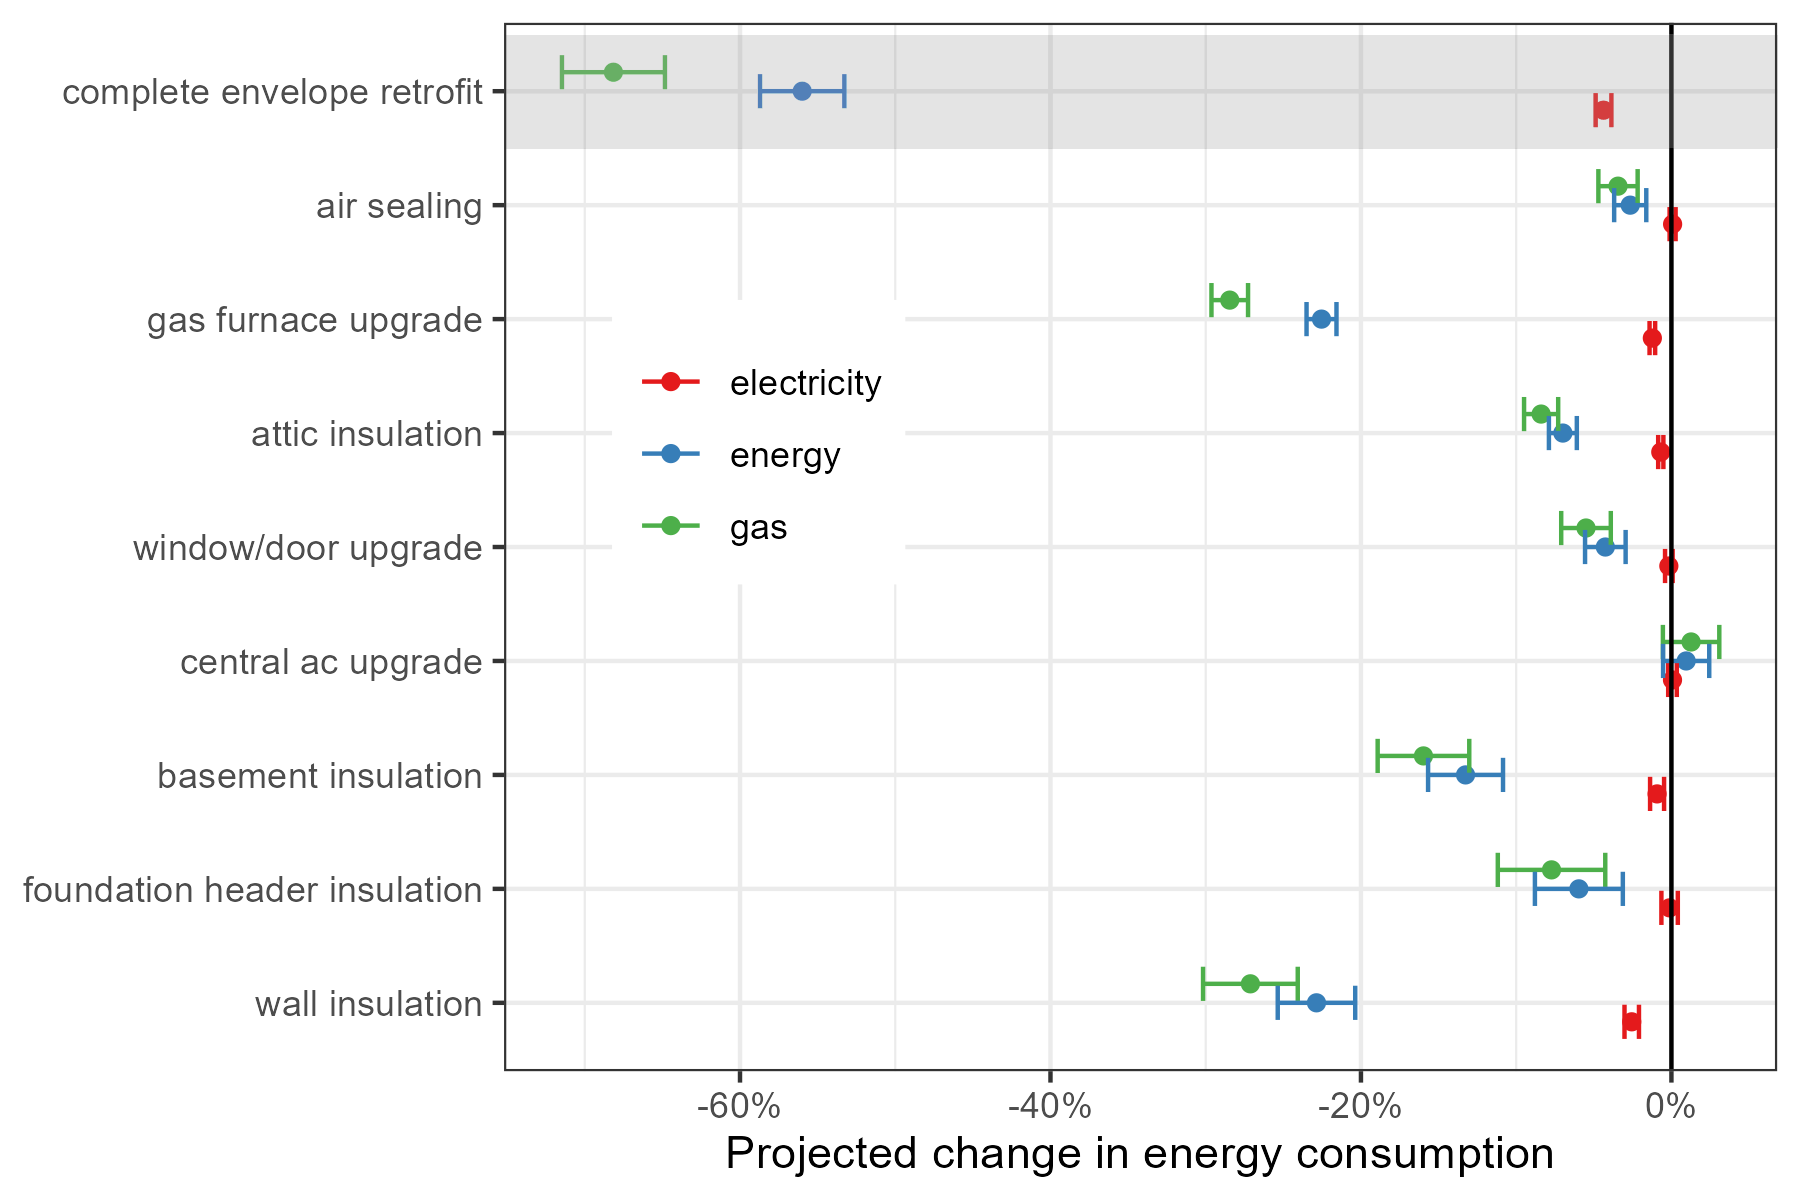
\includegraphics[width=\linewidth]{../output_figures_tables/projected_es_mbm}
\end{frame}

\begin{frame}{Realization rates}
	Overall realization rate table. This is based on estimation in logs. THere is a table based on estimation in levels that can go in Appendix.
	
	
\begin{tabular}{lccc}
   \tabularnewline\midrule\midrule
   Dependent Variables:                                & log(gas)       & log(elec)             & log(energy)\\
   Model:                                              & (1)            & (2)                   & (3)\\
   \midrule \emph{Variables} &   &   &  \\
   as.numeric(treated\_post) $\times$ delta\_gas    & 0.6055$^{***}$ &                       &   \\
                                                       & (0.0195)       &                       &   \\
   as.numeric(treated\_post) $\times$ delta\_elec   &                & 0.1226                &   \\
                                                       &                & (0.5118)              &   \\
   as.numeric(treated\_post) $\times$ delta\_energy &                &                       & 0.5464$^{***}$\\
                                                       &                &                       & (0.0276)\\
   \midrule \emph{Fixed-effects} &   &   &  \\
   id                                                  & Yes            & Yes                   & Yes\\
   cons\_date                                         & Yes            & Yes                   & Yes\\
   \midrule \emph{Fit statistics} &   &   &  \\
   Observations                                        & 3,165,406      & 3,208,330             & 3,176,199\\
   R$^2$                                               & 0.84913        & 0.47322               & 0.78446\\
   Within R$^2$                                        & 0.00417        & $4.62\times 10^{-7}$ & 0.00258\\
   \midrule\midrule\multicolumn{4}{l}{\emph{Clustered (id \& cons\_date) standard-errors in parentheses}}\\
   \multicolumn{4}{l}{\emph{Signif. Codes: ***: 0.01, **: 0.05, *: 0.1}}\\
\end{tabular}



\end{frame}

\begin{frame}{Realization rates measure by measure}
	Here is the realization rate for energy only. The results directory also contains a figure separated by energy type.
	
	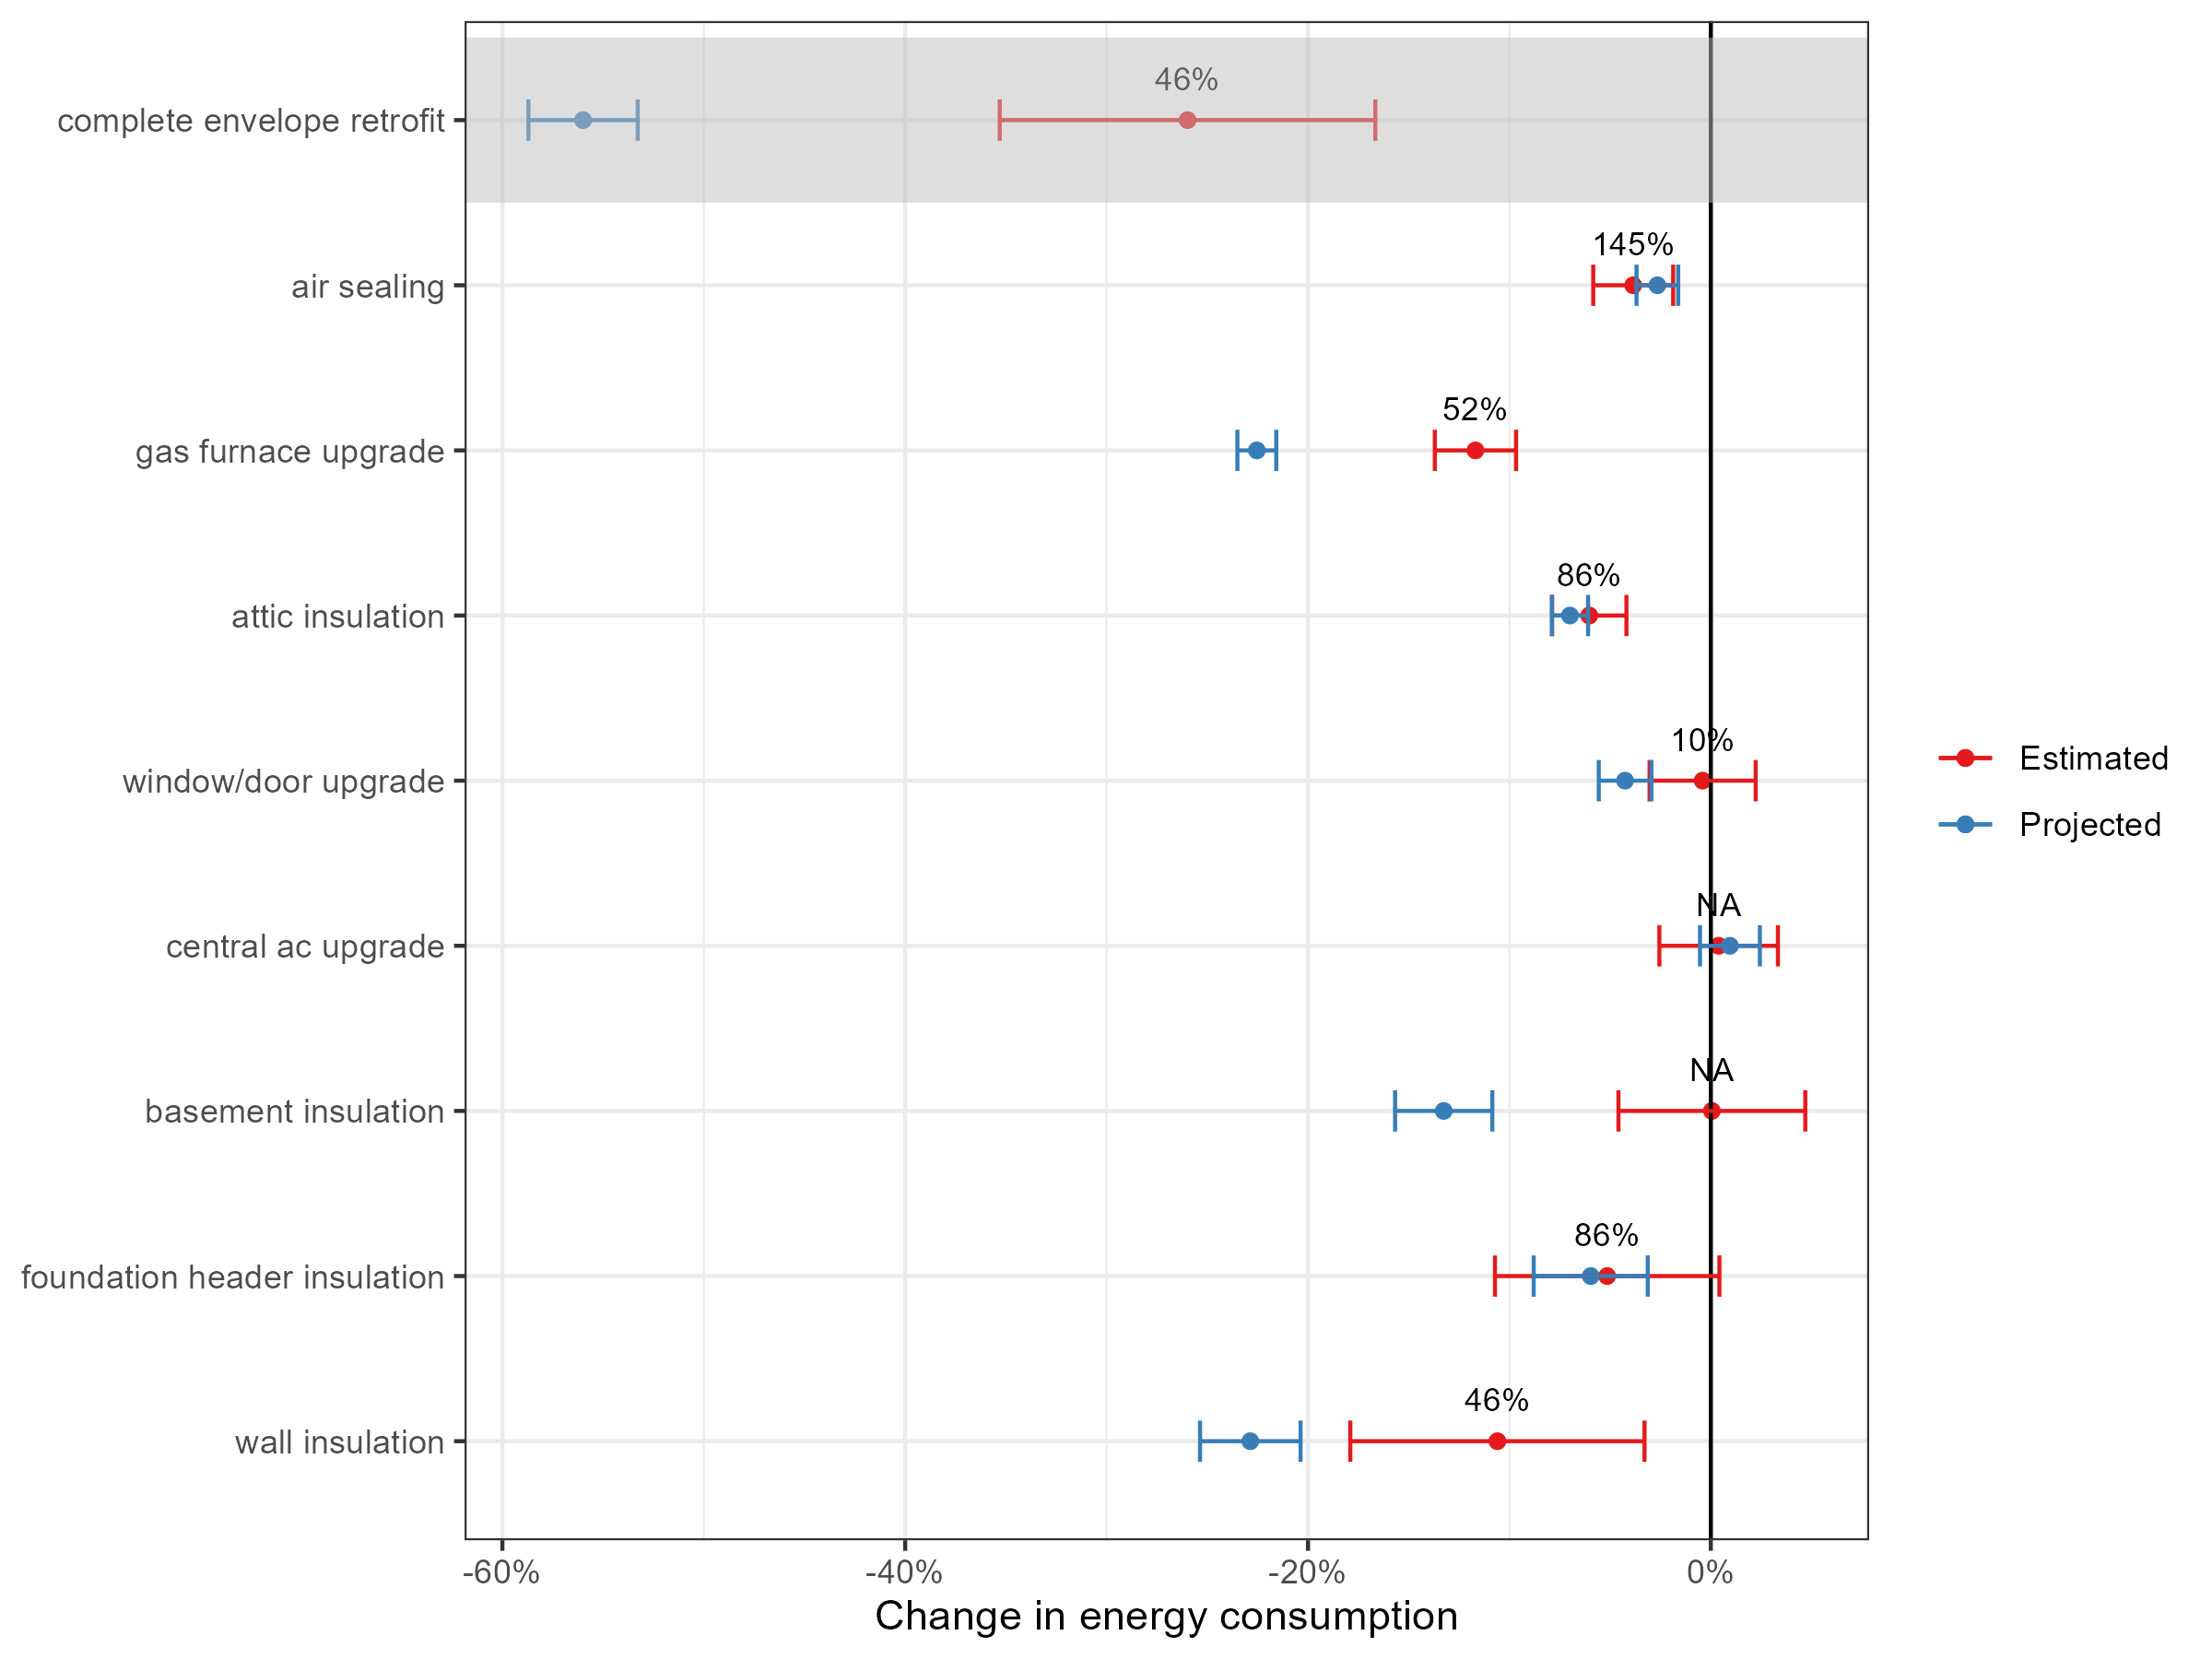
\includegraphics[width=\linewidth]{../output_figures_tables/mbm_realization_rate_all_energy}
\end{frame}

\begin{frame}{Dollar savings}
	As we discussed, we calculate the average rebate in dollars. We calculate the \textit{annual} projected savings and the \textit{annual} realized savings. We divide the average rebate by the average annual savings (both realized and projected).	
	\tiny
	% latex table generated in R 4.2.2 by xtable 1.8-4 package
% Fri Jun 23 14:00:20 2023
\begin{table}[ht]
\centering
\begin{tabular}{rrrr}
  \hline
 & average\_rebate & dollar\_per\_annual\_gj\_realized & dollar\_per\_annual\_gj\_projected \\ 
  \hline
1 & 1016.73 & 48.53 & 22.41 \\ 
   \hline
\end{tabular}
\end{table}

\end{frame}

\begin{frame}{Dollar savings measure by measure}
	\tiny
	% latex table generated in R 4.2.2 by xtable 1.8-4 package
% Thu Oct 26 14:03:17 2023
\begin{table}[ht]
\centering
\begin{tabular}{rlrrrrrrr}
  \hline
 & measure & average\_rebate & savings & projected\_savings & dollar\_per\_annual\_gj\_realized & dollar\_per\_annual\_gj\_projected & dollar\_bill\_saving\_projected & dollar\_bill\_saving\_realized \\ 
  \hline
1 & air\_sealing & 87.62 & 6.69 & 4.57 & 13.09 & 19.18 & 27.31 & 40.03 \\ 
  2 & bsmt\_insulation & 48.65 &  & 27.87 &  & 1.75 & 166.65 &  \\ 
  3 & ceiling\_insulation & 646.25 & 7.61 & 13.11 & 84.90 & 49.30 & 78.40 & 45.52 \\ 
  4 & fnd\_header & 7.38 &  & 8.80 &  & 0.84 & 52.61 &  \\ 
  5 & natural\_gas\_furnace & 489.53 & 15.32 & 37.16 & 31.95 & 13.17 & 222.21 & 91.63 \\ 
  6 & walls\_insulation & 122.80 & 15.21 & 62.39 & 8.07 & 1.97 & 373.12 & 90.95 \\ 
  7 & windowsand\_doors & 108.01 &  & 7.39 &  & 14.62 & 44.19 &  \\ 
   \hline
\end{tabular}
\end{table}

\end{frame}

\end{document}